The example below shows how to use the HyEQ solver to simulate a bouncing ball.

\begin{example}{bouncing ball with Lite HyEQ Solver}
\label{ex:bblite} Consider the hybrid system model for the bouncing ball with data given in \IfSAE{Example~1.1 in the instructions file}{Example~\ref{ex:bb}}.

For this example, we consider the ball to be bouncing on a floor at zero height. The constants for the bouncing ball system are $\gamma = 9.81$ and $\lambda=0.8$.
The following procedure is used to simulate this example in the Lite HyEQ Solver:
\begin{itemize}
\item Inside the MATLAB script {\tt run.m}, initial conditions, simulation horizons, a rule for jumps, ode solver options, and a step size coefficient are defined. The function {\tt HyEQsolver.m} is called in order to run the simulation, and a script for plotting solutions is included.
\item Then the MATLAB functions {\tt f.m, C.m, g.m, D.m} are edited according to the data given above.
\item Finally, the simulation is run by clicking the run button in {\tt run.m} or by calling {\tt run.m} in the MATLAB command window.
\end{itemize}

\begin{figure}[ht]
\begin{center}
\subfigure[Height \label{fig:lite-1}]
{
  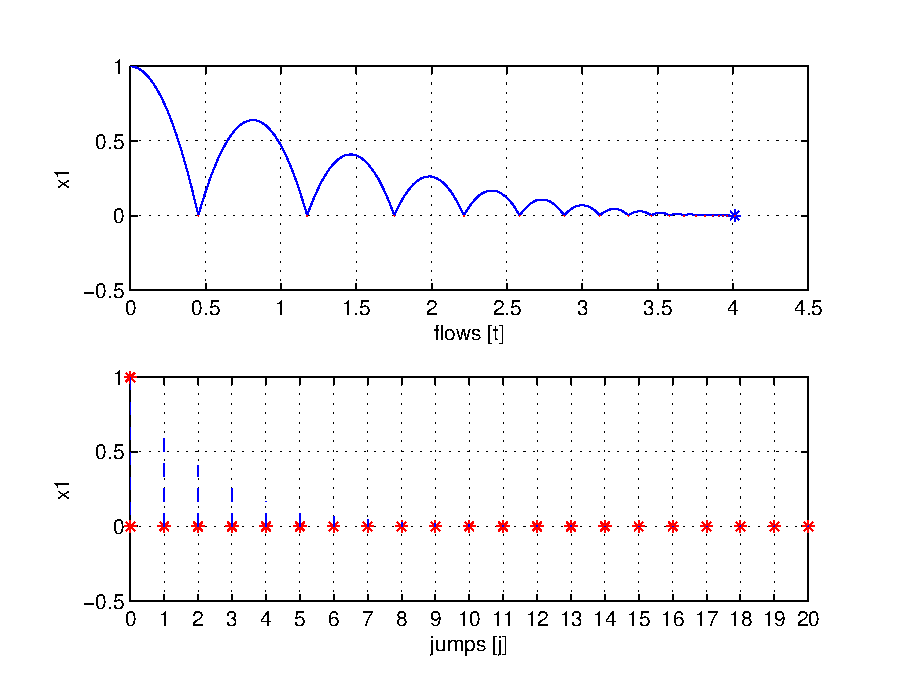
\includegraphics[width=0.48\textwidth]{figures/Examples/FlowsAndJumps1lite}
}
\hfill
\subfigure[Velocity \label{fig:lite-2}]
{
  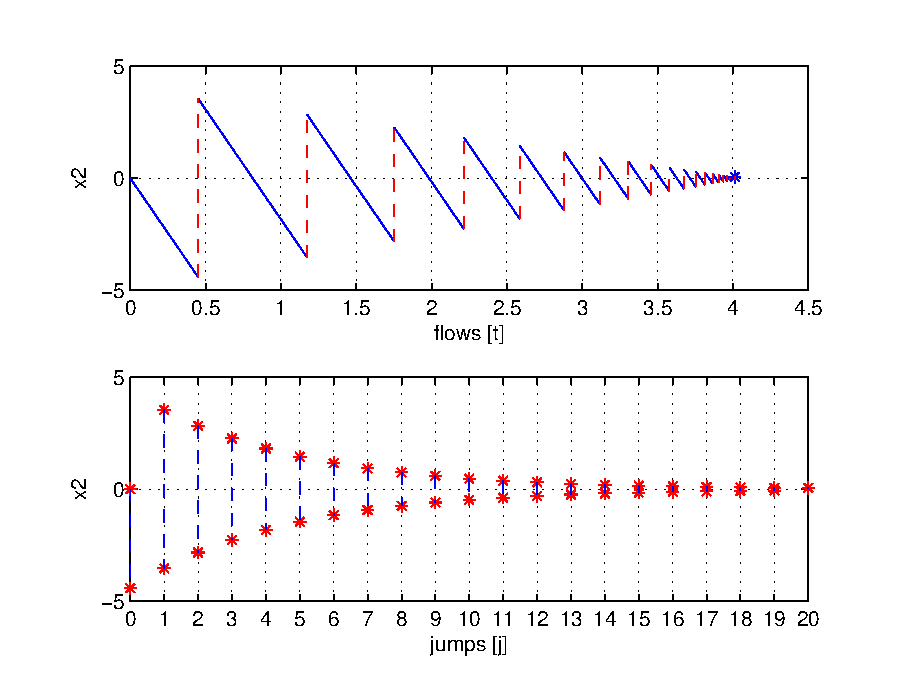
\includegraphics[width=0.48\textwidth]{figures/Examples/FlowsAndJumps2lite}
}
\end{center}
\caption{Solution of Example \ref{ex:bblite}
  %TODO: Replace figures with labels formatted using LaTeX interpreter.
}
\end{figure}

\begin{figure}[ht]
  \begin{center}
  \psfrag{t}[c]{$t$}
  \psfrag{j}[c]{$j$}
  \psfrag{x1}[c]{$x_1$}
    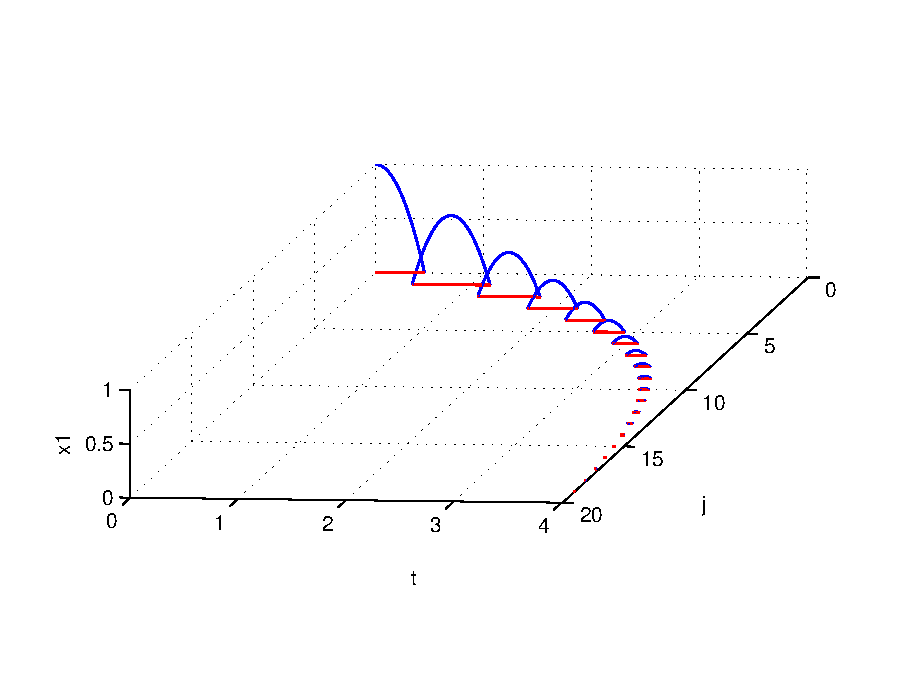
\includegraphics[width=.8\textwidth]{figures/Examples/HybridArclite}
    \caption{Hybrid arc corresponding to a solution of Example~\ref{ex:bblite}: height
      %TODO: Replace figures with labels formatted using LaTeX interpreter.
    }
    \label{fig:lite-3}
  \end{center}
\end{figure}

Example code for each of the MATLAB files {\tt run.m, f.m, C.m, g.m,} and {\tt D.m} is given below.\\
%\scriptsize

% Set the location for MATLAB files included via the "\code" command.
\codeLocation{Matlab2tex_1_2}

\code{run.m}
\code{f.m}
\code{C.m}
\code{g.m}
\code{D.m}

A solution to the bouncing ball system from 
$x(0,0)=[1,0]^\top$ and with 
$TSPAN = [0 \hspace{2mm} 10], JSPAN = [0 \hspace{2mm} 20]$, $rule =1$, 
is depicted in Figure~\ref{fig:lite-1} (height) 
and Figure~\ref{fig:lite-2} (velocity).  
Both the projection onto $t$ and $j$ are shown. 
Figure~\ref{fig:lite-3} depicts the corresponding hybrid arc for the position state.

For MATLAB files of this example, 
see \IfSAE{Examples/Example\_\ref{ex:bblite}}{Examples/Example\_1.2}.



\end{example}
